\documentclass[12pt]{IEEEtran}
\usepackage{../../../template}
\title{Knots and Topological Transformations in Vibrating Chains}
\begin{document}
\maketitle

\begin{abstract}
    This experiment was conducted to investigate knot and topological transformation in vibrating chains. The dependence of unknotting time on chain length and frequency were separately examined. The conclusions for chain length were inconclusive due to insufficient measurements. As for frequency, it is theorized that unknotting time has a sinusoidal dependence on frequency. More experimentation is needed to further verify this. These results can be used to better understand the behaviour of knots, which are involved in a variety of physical processes, e.g. DNA replication, polymer formation, where it is difficult to directly observe knotting behaviour for various reasons.
\end{abstract}

\section{Introduction}

The dynamics of knots in granular chains vibrating on a plate is studied in this experiment. Understanding this phenomenon is crucial in understanding many biophysical processes or the structural properties of many materials, but it is very difficult to study these processes directly~\cite{manual}. This is where this experiment comes in. The phenomenon was modeled with knots tied with a chain of beads and placed on a vibrating plate. Unknotting behaviour could be learned from average unknotting time given different parameters. Note that there is a need to use average unknotting time, since unknotting time follows a distribution, so many measurements of the same setup needs to be taken to produce data with acceptable uncertainties. \\
In the first part, I attempted to verify the predictions of Ben-Naim et al.~\cite{bennaim}. It states that for a trefoil knot, which is the simplest knot which overlaps itself exactly 3 times, average unknotting time depends on chain length based on the following equation.

\begin{equation}
    t_{avg} = t_0(N - N_0)^\delta
\end{equation}

where $N$ is the chain length, $N_0$ is the knot length, and $t_0, \delta$ are values to be determined. It is predicted~\cite{bennaim} that $\delta = 2 \pm 0.1$. A trivialisation of the theory is that the two outermost overlaps travel along the chain bead by bead for every vibration, and that this can be approximated by a random walk. Therefore, the only parameter which matters is the $(N - N_0)$, the length which the knot has to travel before it is unraveled. \\

In the second part of the experiment, I investigated the dependence of unknotting time on frequency. There is no well-developed theory for this, so the goal was to take enough data to fit a simple equation, which could then be used as a first-order approximation for unknotting times within the tested frequencies.

\section{Experimental Techniques}

Techniques below are taken from the laboratory write-up~\cite{manual}.

\subsection{Methods and Materials}

The chains used in the experiment are ball chains consisting of hollow metal spheres connected through rods. Specifically, the ball chain used has a length of 105 spheres, with each bead having a measured diameter of $2.5\pm0.5\unit{mm}$. Its density is $0.0352 \pm 0.0005$ g/bead. The shaker is an aluminium plate securely attached to a magnetically driven SP10 Sub-Woofer speaker, driven by a signal/frequency generator through a power amplifier. An MMA 1220 accelerometer is attached to the bottom of the plate, an an oscilloscope is used to record the voltage readings, which are used to calculate for acceleration.

\subsection{Procedures}

Throughout the experiment, there was a need to find the average unknotting time given the certain conditions. For the same conditions, at least 30 measurements were taken. In each measurement, the vibrating plate was turned on with the chain placed on it. The correct frequency was set, and then the amplitude was adjusted until the desired maximum acceleration was produced. For convenience, the initial positions of the knot were marked with a pen, so the same length of knot can be retied over and over. \\
Individual measurements took place upon completion of initial set up. In each measurement, the knot was tied with help of the markings, and was placed in the centre of the plate. The same method was used to complete the knot the reduce external factors. The waveform generator and the stopwatch were triggered simultaneously to reduce systematic timing errors. \\
Throughout the experiment, voltage was set to a constant value of $\Delta V = 1.48\unit{V}$, which corresponds to an acceleration of $29.0 \pm 0.05 \unit{m.s^{-2}}$ as calculated using the accelerometer specifications~\cite{accelerometer}. Frequency, chain length, and number of measurements are as follows

\begin{table}
    \begin{tabular}{|c|c|c|}
        \hline
        Frequency (Hz) & Chain Length (Balls) & Number of Measurements \\
        \hline\hline
        11 & 34 & 40 \\
        \hline
        12 & 34 & 30 \\
        \hline
        13 & 34 & 30 \\
        \hline
        14 & 34 & 30 \\
        \hline
        15 & 10 & 30 \\
        \hline
        15 & 34 & 30 \\
        \hline
        15 & 50 & 30 \\
        \hline
        15 & 78 & 68 \\
        \hline
        16 & 34 & 30 \\
        \hline
        17 & 34 & 30 \\
        \hline
        19 & 34 & 30 \\
        \hline
    \end{tabular}
    \caption{Variables of Measurements Taken}
\end{table}

\section{Results and Discussion}

In the following section, we use "measurements" to denote the individual measurements of unknotting time. A "data point" is the average of measurements given the same conditions, i.e. $t_{avg}$.

\subsection{Experimental Value of $\delta$}

\begin{figure}[h]
    \centering
    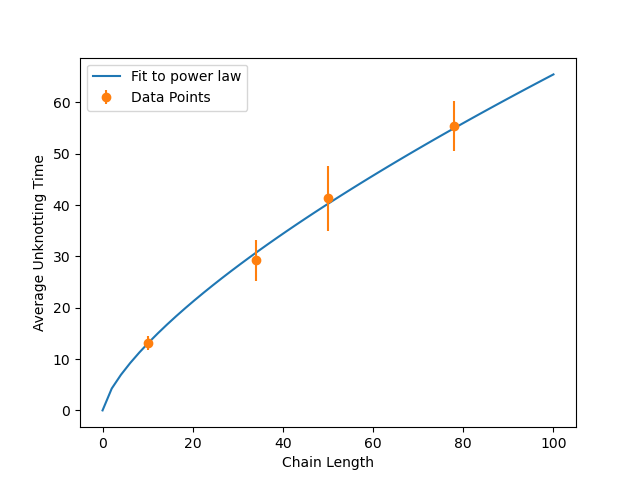
\includegraphics[scale=0.5]{part1_plot.png}
    \caption{Fit of $t_{avg} = t_0(N - N_0)^\delta$}
\end{figure}

\begin{figure}[h]
    \centering
    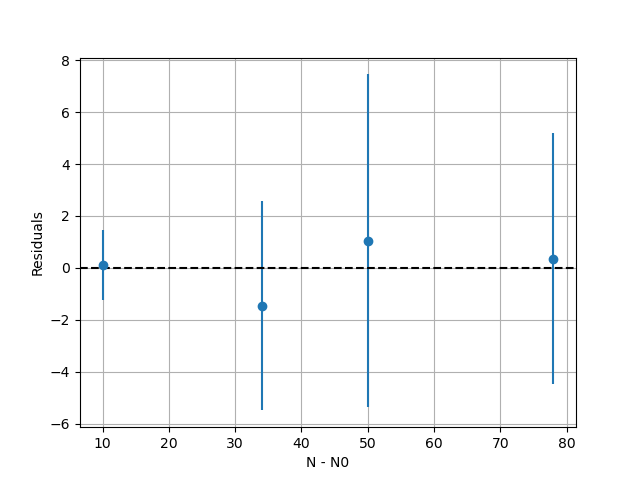
\includegraphics[scale=0.5]{part1_res.png}
    \caption{Residuals for the Power Law}
\end{figure}

A non-linear least squares fit~\cite{curvefit} gives $\delta = 0.7 \pm 0.07$, which is far from the theoretical predicted value of 2, taking uncertainty into account. The residuals are all within uncertainty, but the reduced $\chi^2$ value is $0.086$, which is much lower than expected. This implies overfitting; it may be beneficial to take more data points at different values of $(N - N_0)$. Moreover, from the residuals, it is also possible that the uncertainties were too large to begin with, which createes the false impression that the residuals are small. In this case, more measurements can be taken per data point to reduce uncertainties. \\
A possibility is that the predicted value of 2 is incorrect, perhaps due to invalid assumptions in the theoretical model. However, the authors of the paper also supported the value (Fig~\ref{theoretical}) with 9 data points, each consisting of at least 400 measurements, both of which are greater than that of this experiment. As such, it is more likely that the shortcomings as described above have contributed to the deviation in $\delta$.

\begin{figure}[h]
    \centering
    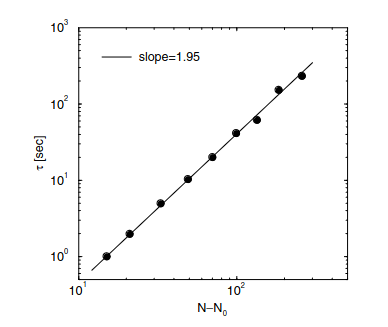
\includegraphics[scale=0.5]{theoretical.png}
    \caption{Fit to Power Law by Ben-Naim et al.~\cite{bennaim}}\label{theoretical}
\end{figure}

\subsection{Part 2}

\begin{figure}[h]
    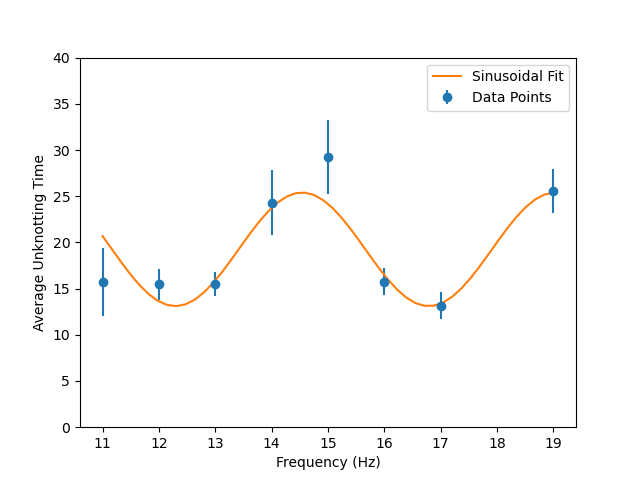
\includegraphics[scale=0.5]{part2_plot.png}
    \caption{Unknotting Time versus Frequency}\label{part2data}
\end{figure}

Unknotting time versus frequency is as shown in Fig~\ref{part2data}. Based on the data, it was theorized that there could be a sinusoidal relationship( Eq~\ref{guess}) between both. The same non-linear least squares fit yielded values of $a = 6 \pm 1\unit{s}, b = 1.4 \pm 1\unit{s}, c = -6 \pm 1, d = 19.3 \pm 0.9\unit{s}$.

\begin{equation}\label{guess}
    t_{avg} = a\sin(bf + c) + d
\end{equation}

\begin{figure}[h]
    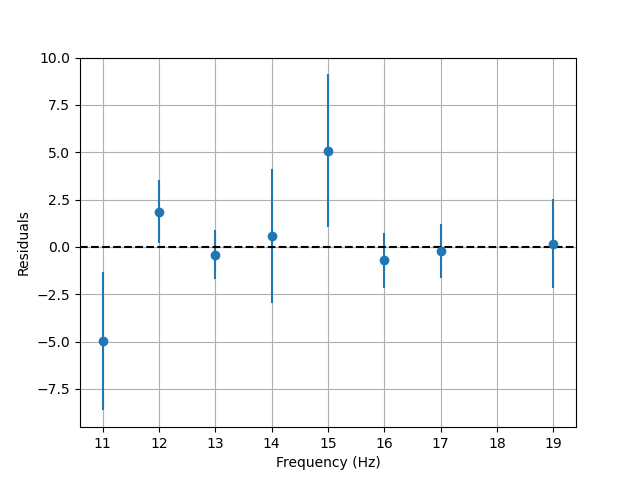
\includegraphics[scale=0.5]{part2_res.png}
    \caption{Residuals for Unknotting Time versus Frequency}\label{part2res}
\end{figure}

The reduced $\chi^2$ was $1.28$, which was close to 1, indicating a good fit. The residuals (Fig~\ref{part2res}) had no discernable patterns, hinting there were no significant features uncaptured by the fit. Most of the errors were also within uncertainty. \\
More experimentation is required to verify this theory. There needs to be a theoretical model that justifies this behaviour and predicts testable results, which can be verified with further experiments. In terms of experimentation, the uncertainties are too large, and each data point can benefit from more measurements. Data should also be taken for a wider range of frequencies to ensure this is a global phenomenon. If possible, chain length, material properties, and amplitude can also be varied, to further study how these variables affect the parameters $a,b,c,d$, and to see if they possibly verify theoretical predictions for the relationships between parameters and those properties.

\subsection{Uncertainties}

The sources of uncertainties mostly apply for time. There was statistical error from the distribution of unknotting time, human error when measured time was consistently delayed by reaction time, and systematic error from starting the stopwatch and waveform generator at the same time, since there may be a delay between that and the vibration of the plate. However, the first error was on the order of seconds, which the remaining errors were both within a second. Therefore, we consider only statistical uncertainties in the experiment. Uncertainties were then computed as the standard error of the mean, $\frac{\sigma}{\sqrt{n}}$, where $\sigma$ is the sample standard deviation $\sigma = \sqrt{\frac{\sum_i (x_i - \bar x)^2}{n-1}}$. \\
Many significant figures were provided by the oscilloscope, yet measurements relied on human estimations of the lines going through the maximum and minimum. Three significant figures were taken, and the error was taken to be half of the final significant figure. The waveform generator provided more than five significant figures for frequency, so its values were taken to be exactly correct, in light of the larger sources of error for other variables.

\section{Conclusion}

This experiment shows that the power law as derived by Ben-Naim et al. may not be global. Specifically, it is possible that $\delta$ depends on more than just the type of knot, meaning $\delta \approx 2$ may not hold for all trefoil knots. This points out a need to rigorously test existing theory for various material properties. It also hints that average unknotting time may have a sinusoidal dependence on vibration frequency, at least on a local level. More experimentation could provide more insight on this phenomenon, and theoretical models can be developed to help understand the complex processes as described in the introduction.

\bibliography{refs.bib}{}
\bibliographystyle{IEEEtran}
\end{document}
